\begin{frame}
\titlepage
\end{frame}

% слайд с инофрмацией об авторах
% кратко написать о себе, оставить контанты
% может быть надо встравить фотки какие то
\begin{frame}{Информация об авторах курса}

\begin{center}
\begin{tabular}{ c c  }
 Кондаков Данила Евгеньевич  (kondakovde@modeltech.ru)  & 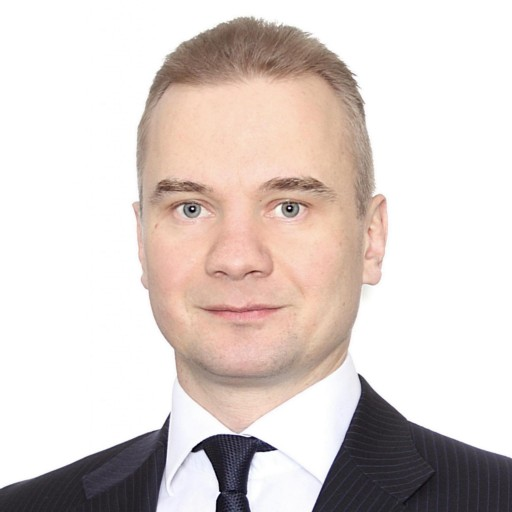
\includegraphics[scale=0.2]{fig/kondakov.jpeg}  \\ 
 Хабибуллин Ринат Альфредович  (khabibullin.ra@gubkin.ru) &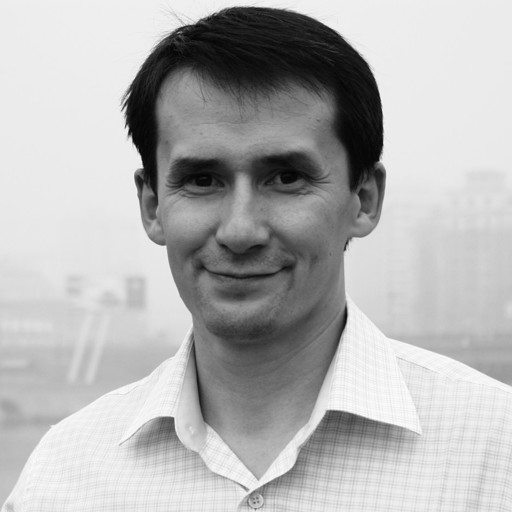
\includegraphics[scale=0.15]{fig/khabibullin.jpeg}
\end{tabular}
\end{center}

%\begin{itemize}

%    \item Кондаков Данила Евгеньевич \\ (kondakovde@modeltech.ru) 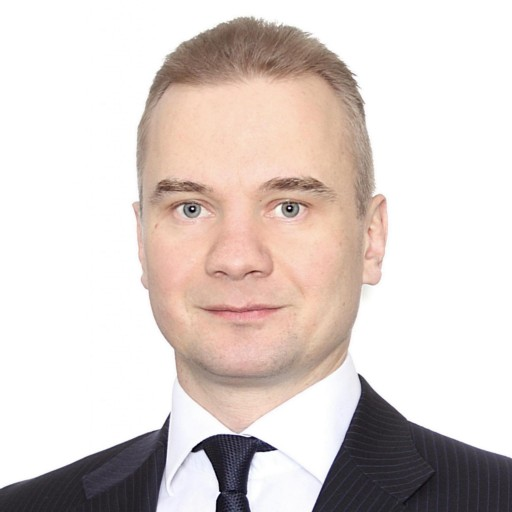
\includegraphics[scale=0.2]{fig/kondakov.jpeg}
%    \item Хабибуллин Ринат Альфредович (khabibullin.ra@gubkin.ru)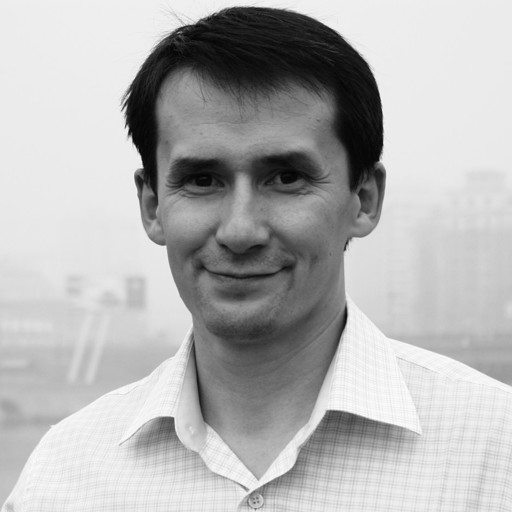
\includegraphics[scale=0.15]{fig/khabibullin.jpeg}
%\end{itemize}
    
\end{frame}

% слайд с описанием 
% чтобы и самим не запутаться - что хотим донести то
\begin{frame}{Описание курса}
\begin{itemize}
    \item Цели курса - получить представление об основных ключевых факторах влияющих на эффективность разработки месторождений нефти, изучить цепочку создания ценности при разработке месторождений.
    \item Инструмент изучения - разбор задачи интегрированного концептуального проектирования разработки месторождений.
    \item Задачи курса - получить навыки проведения инженерных расчетов ключевых факторов разработки с использованием компьютерных моделей.
    \item Курс носит практическую направленность - лучше изучать разработку через расчеты! ("разработчикам платят за цифры"!)
\end{itemize}
\end{frame}

\begin{frame}{Сайт поддержки курса \href{rienm.ru}{rienm.ru}}
\begin{center}
 \textbf{ \href{rienm.ru}{rienm.ru}   }
\end{center}
 
\begin{itemize}
    \item Курс "ИРНП-2020", "Основы интегрированной разработки нефтяных проектов"
    \item На сайте - дополнительные материалы, инструкции, задания и пр.
    \item Надо зарегистрироваться и подписаться на курс. ключевое слово для записи на курс "ISKRA"
\end{itemize}
    
\end{frame}

% слайд содержание курса
%   - основные разделы по которым будет построен курс
\begin{frame}{Содержание курса}
\begin{enumerate}
    \item Введение. Основы разработки нефтяных месторождений.
    \item Заканчивание, кустование и бурение скважин.
    \item Выбор скважинного оборудования и поверхностного обустройства.
    \item Финансово-экономическая модель.
    \item Оптимизация интегрированного концептуального проекта. 
    \item Работа над проектным заданием.
\end{enumerate}
\end{frame}

% Блок вводных слайдов, которые описывают задачу интегрированного концептуального проектирования
%
\begin{frame}{Жизненный цикл месторождения. Проект разработки}
\begin{center}



\tikzset{every picture/.style={line width=0.75pt}} %set default line width to 0.75pt        

\begin{tikzpicture}[x=0.75pt,y=0.75pt,yscale=-1,xscale=1]
%uncomment if require: \path (0,300); %set diagram left start at 0, and has height of 300

%Pentagon Arrow [id:dp3101695977599498] 
\draw  [fill={rgb, 255:red, 208; green, 227; blue, 249 }  ,fill opacity=1 ] (9,30) -- (54.88,30) -- (90.88,71.7) -- (54.88,113.4) -- (9,113.4) -- cycle ;
%Chevron Arrow [id:dp07604580827828711] 
\draw  [fill={rgb, 255:red, 208; green, 227; blue, 249 }  ,fill opacity=1 ] (63.84,30.19) -- (145.4,30.23) -- (181.8,71.94) -- (145.33,113.6) -- (63.76,113.56) -- (100.24,71.89) -- cycle ;
%Chevron Arrow [id:dp5811273998449972] 
\draw  [fill={rgb, 255:red, 208; green, 227; blue, 249 }  ,fill opacity=1 ] (153.74,30.2) -- (280.6,30.26) -- (316.7,71.96) -- (280.53,113.62) -- (153.66,113.55) -- (189.83,71.89) -- cycle ;
%Chevron Arrow [id:dp9203859009724674] 
\draw  [fill={rgb, 255:red, 208; green, 227; blue, 249 }  ,fill opacity=1 ] (286.64,30.19) -- (397.4,30.25) -- (433.1,71.95) -- (397.33,113.61) -- (286.56,113.56) -- (322.33,71.89) -- cycle ;
%Chevron Arrow [id:dp9845040169134129] 
\draw  [fill={rgb, 255:red, 208; green, 227; blue, 249 }  ,fill opacity=1 ] (403.94,30.19) -- (509.4,30.25) -- (543.9,71.95) -- (509.33,113.61) -- (403.86,113.56) -- (438.44,71.89) -- cycle ;

% Text Node
\draw (45,71.76) node   [align=left] {Разведка};
% Text Node
\draw (131.17,71.83) node   [align=left] {Оценка \\запасов};
% Text Node
\draw (249.4,71.89) node   [align=left] {Проектирование};
% Text Node
\draw (373.6,71.89) node   [align=left] {Эксплуатация};
% Text Node
\draw (488.5,71.89) node   [align=left] {Ликвидация};


\end{tikzpicture}


Где на схеме наш курс?    

Сравните с проектным подходом



\tikzset{every picture/.style={line width=0.75pt}} %set default line width to 0.75pt        

\begin{tikzpicture}[x=0.75pt,y=0.75pt,yscale=-1,xscale=1]
%uncomment if require: \path (0,300); %set diagram left start at 0, and has height of 300

%Pentagon Arrow [id:dp45739470564915163] 
\draw  [fill={rgb, 255:red, 239; green, 234; blue, 234 }  ,fill opacity=1 ] (9,157.75) -- (70.33,157.75) -- (101,170.87) -- (70.33,183.98) -- (9,183.98) -- cycle ;
%Chevron Arrow [id:dp7716941966146128] 
\draw  [fill={rgb, 255:red, 239; green, 234; blue, 234 }  ,fill opacity=1 ] (78.84,158.16) -- (170.33,158.18) -- (202.33,171.09) -- (170.25,183.98) -- (78.75,183.97) -- (110.83,171.07) -- cycle ;
%Chevron Arrow [id:dp4248711020529512] 
\draw  [fill={rgb, 255:red, 239; green, 234; blue, 234 }  ,fill opacity=1 ] (178.07,158.17) -- (281.89,158.19) -- (313.66,171.1) -- (281.81,184) -- (177.99,183.98) -- (209.84,171.08) -- cycle ;
%Chevron Arrow [id:dp6674834695666102] 
\draw  [fill={rgb, 255:red, 239; green, 234; blue, 234 }  ,fill opacity=1 ] (291.3,158.44) -- (406,158.46) -- (437.76,171.22) -- (405.92,183.98) -- (291.22,183.96) -- (323.06,171.2) -- cycle ;
%Chevron Arrow [id:dp36707241342832] 
\draw  [fill={rgb, 255:red, 239; green, 234; blue, 234 }  ,fill opacity=1 ] (414.27,158.44) -- (522.33,158.46) -- (554.23,171.35) -- (522.25,184.24) -- (414.19,184.22) -- (446.16,171.34) -- cycle ;

% Text Node
\draw (49.5,170.87) node  [font=\scriptsize] [align=left] {Поиск};
% Text Node
\draw (152.17,170.87) node  [font=\scriptsize] [align=left] {Оценка };
% Text Node
\draw (249.9,170.87) node  [font=\scriptsize] [align=left] {Выбор};
% Text Node
\draw (372.77,170.87) node  [font=\scriptsize] [align=left] {Определение};
% Text Node
\draw (488.5,170.87) node  [font=\scriptsize] [align=left] {Реализация};


\end{tikzpicture}

\end{center}

%Тут надо будет показать картинки жизненного цикла от разведки через разработку и ликвидацию месторождения. 
%На картинке показать где актуальная задача проектирования. 

\end{frame}

\begin{frame}{Моделирование в разработке нефтяных проектов}
\begin{center}
    Попробуйте ответить на вопросы ниже
\end{center}
\begin{itemize}
    \item Какова роль моделирования в нефтяных проектах? 
    \item Цели и задачи моделирования?
    \item Проектирование и моделирование как связаны?
    \item Управление месторождением и моделирование как связаны?
\end{itemize}
 
\end{frame}

\begin{frame}{Некоторые принципы моделирования}
    \begin{itemize}
        \item Знание некоторых принципов легко возмещает незнание некоторых фактов
        \item Все модели неверны - но некоторые полезны
        \item Модель должна быть как можно проще, но не проще чем необходимо
        \item Видеть лес за деревьями 
    \end{itemize}
\end{frame}

\begin{frame}{Информационный поток принятия решений}
\begin{center}
    




\tikzset{every picture/.style={line width=0.75pt}} %set default line width to 0.75pt        

\begin{tikzpicture}[x=0.75pt,y=0.75pt,yscale=-1,xscale=1]
%uncomment if require: \path (0,298); %set diagram left start at 0, and has height of 298

%Pentagon Arrow [id:dp05783596747150732] 
\draw  [fill={rgb, 255:red, 228; green, 242; blue, 214 }  ,fill opacity=1 ] (35,70.5) -- (122,70.5) -- (180,105.75) -- (122,141) -- (35,141) -- cycle ;
%Pentagon Arrow [id:dp3515872489371136] 
\draw  [fill={rgb, 255:red, 228; green, 242; blue, 214 }  ,fill opacity=1 ] (193,70.5) -- (280,70.5) -- (338,105.75) -- (280,141) -- (193,141) -- cycle ;
%Pentagon Arrow [id:dp36029876570649744] 
\draw  [fill={rgb, 255:red, 228; green, 242; blue, 214 }  ,fill opacity=1 ] (352,70.5) -- (439,70.5) -- (497,105.75) -- (439,141) -- (352,141) -- cycle ;

% Text Node
\draw (97,105.75) node   [align=left] {Данные};
% Text Node
\draw (257.5,105.75) node   [align=left] {Информация};
% Text Node
\draw (412.5,105.75) node   [align=left] {Решения};


\end{tikzpicture}



Принятие решений - задача инженерной деятельности
\end{center}
\begin{itemize}
    \item Данные - то, что записано и/или сохранено
    \item Информация - то, что подготовлено для принятие решений, интерпретировано
    \item Решение - необратимая трата ресурсов, времени, сил, средств
\end{itemize}{}

\end{frame}

\begin{frame}{Моделирование - инструмент принятия решений}
\begin{center}
    


\tikzset{every picture/.style={line width=0.75pt}} %set default line width to 0.75pt        

\begin{tikzpicture}[x=0.75pt,y=0.75pt,yscale=-1,xscale=1]
%uncomment if require: \path (0,298); %set diagram left start at 0, and has height of 298

%Pentagon Arrow [id:dp05783596747150732] 
\draw  [fill={rgb, 255:red, 228; green, 242; blue, 214 }  ,fill opacity=1 ] (35,70.5) -- (122,70.5) -- (180,105.75) -- (122,141) -- (35,141) -- cycle ;
%Pentagon Arrow [id:dp3515872489371136] 
\draw  [fill={rgb, 255:red, 228; green, 242; blue, 214 }  ,fill opacity=1 ] (193,70.5) -- (280,70.5) -- (338,105.75) -- (280,141) -- (193,141) -- cycle ;
%Pentagon Arrow [id:dp36029876570649744] 
\draw  [fill={rgb, 255:red, 228; green, 242; blue, 214 }  ,fill opacity=1 ] (352,70.5) -- (439,70.5) -- (497,105.75) -- (439,141) -- (352,141) -- cycle ;
%Callout Right Arrow [id:dp6519087741930664] 
\draw  [fill={rgb, 255:red, 245; green, 166; blue, 35 }  ,fill opacity=1 ] (116.55,211.51) -- (116.47,176.32) -- (161.18,176.21) -- (161.15,162.14) -- (150.59,162.16) -- (171.66,141) -- (192.82,162.07) -- (182.26,162.09) -- (182.29,176.17) -- (227,176.07) -- (227.08,211.26) -- cycle ;
%Callout Right Arrow [id:dp9343533398145991] 
\draw  [fill={rgb, 255:red, 245; green, 166; blue, 35 }  ,fill opacity=1 ] (267.48,211.14) -- (267.4,176.14) -- (319.55,176.02) -- (319.52,162.02) -- (309.02,162.05) -- (329.98,141) -- (351.02,161.95) -- (340.52,161.98) -- (340.55,175.98) -- (392.71,175.86) -- (392.79,210.86) -- cycle ;
%Shape: Brace [id:dp5722533717787442] 
\draw   (31,217) .. controls (31.01,221.67) and (33.34,224) .. (38.01,223.99) -- (255.01,223.77) .. controls (261.68,223.76) and (265.01,226.08) .. (265.01,230.75) .. controls (265.01,226.08) and (268.34,223.75) .. (275.01,223.74)(272.01,223.75) -- (492.01,223.52) .. controls (496.68,223.51) and (499.01,221.18) .. (499,216.51) ;

% Text Node
\draw (97,105.75) node   [align=left] {Данные};
% Text Node
\draw (257.5,105.75) node   [align=left] {Информация};
% Text Node
\draw (412.5,105.75) node   [align=left] {Решения};
% Text Node
\draw (170.8,192.8) node   [align=left] {Модели};
% Text Node
\draw (333.6,192.8) node   [align=left] {Модели};
% Text Node
\draw (268,244) node   [align=left] {Знание};


\end{tikzpicture}

\end{center}
\begin{itemize}
    \item Инженерные расчеты направлены на принятие решений
    \item Возможные решения - часть инженерной модели
\end{itemize}{}

\end{frame}

\begin{frame}{Интегрированный концептуальный проект}

Интегрированный проект - такой где совместно решаются разномасштабные задачи разработки - фильтрация в пласте, работа скважины, скважинного оборудования и поверхностного обустройства.

Интегрированный концептуальный проект - один из подходов к созданию интегрированных проектов. Сосредотачивается на ключевых решениях разработки - выбор сетки скважины, типа заканчивания скважины, способа подъема жидкости на поверхность, основных узлов поверхностного обустройства.

Цель интегрированного концептуального проекта - принятие решения о "вхождении" в проект? проработка деталей проекта? что-то другое?

%Надо тут пояснить сложность интегрированной задачи - большое количество переменных на каждом этапе и необходиость "сшивки" решений.

\end{frame}




\begin{frame}{Ключевые разделы курса (интегрированного концептуального проекта)}

\begin{center}
    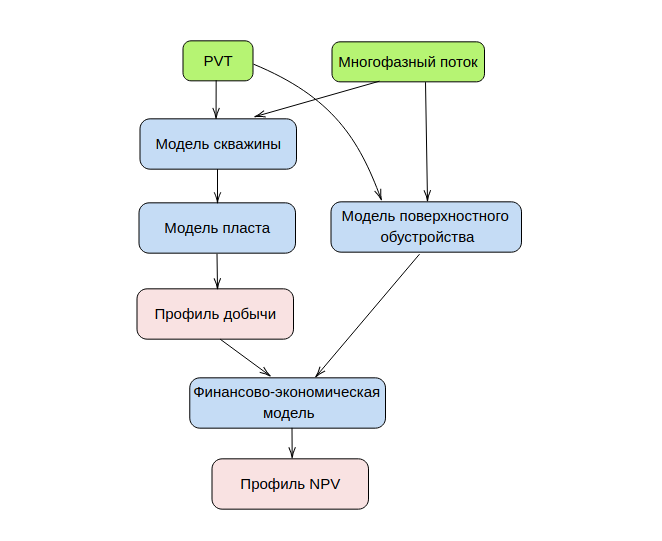
\includegraphics[scale=0.4]{key_topics}
\end{center}

    
\end{frame}




\begin{frame}{Что вы знаете о PVT?}
\begin{columns}
\column{0.8\textwidth}
    \begin{itemize}
        \item Где нефть занимает больший объем – в пласте или на поверхности?
        \item Какие подходы к построению моделей флюидов вы знаете?
        \item Перечислите параметры флюидов которые вы знаете и которые необходимы для моделирования системы добычи
        \item Что такое газовый фактор?
        \item Что надо знать, чтобы определить долю газа в потоке?
        \item Как изменятся свойства флюида после сепарации газа (отделения части газа из потока)?  
    \end{itemize}
\column{0.2\textwidth}
    
\includegraphics[scale=0.3]{fig/question_pic.png}
    \newline
    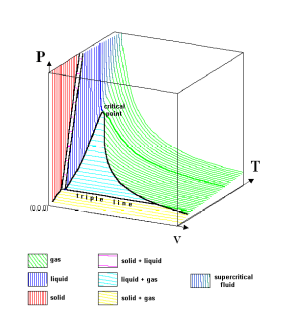
\includegraphics[scale=0.3]{fig/PVT.png}
\end{columns}
\end{frame}



\begin{frame}{PVT упражнение}
\begin{columns}
\column{0.8\textwidth}
    \begin{itemize}
        \item Постройте зависимости газосодержания в нефти, объемного коэффициента нефти, вязкости нефти и давления и температуры
        \item Постройте зависимость доли газа в потоке от давления и температуры
        \item Постройте зависимость давления при которой достигается заданная доля газа в потока от газового фактора и обводненности
        \item*Какие параметры наиболее сильно влияют на значение давления при которой достигается заданная доля газа в потоке (график торнадо)
    \end{itemize}
    Подробное описание задания на сайте rienm.ru
\column{0.2\textwidth}
    
\includegraphics[scale=0.3]{fig/task.png}
    \newline
    
\includegraphics[scale=0.3]{fig/xls.png}
\end{columns}
\end{frame}

\begin{frame}{Гидродинамическое моделирование}
\begin{columns}
\column{0.5\textwidth}
    \begin{center}
        RSO
        \newline
        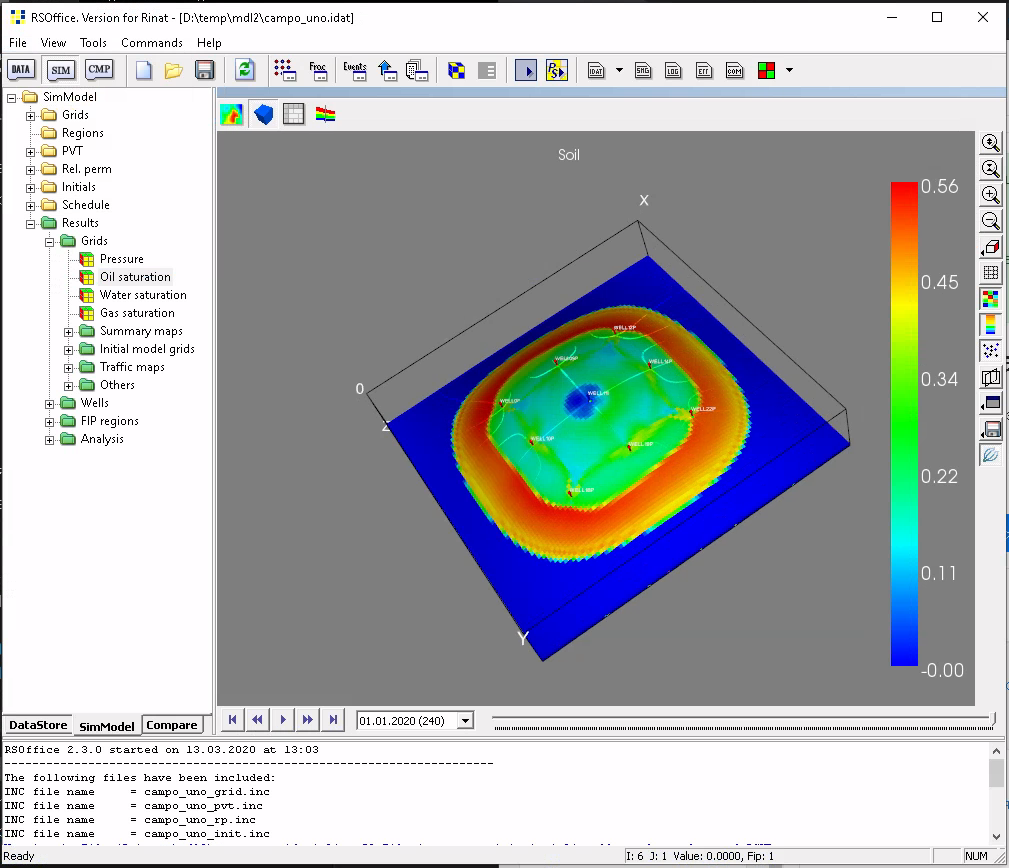
\includegraphics[scale=0.2]{fig/RSO.png}
    \end{center}
\column{0.5\textwidth}
    \begin{center}
        OPM
        \newline
        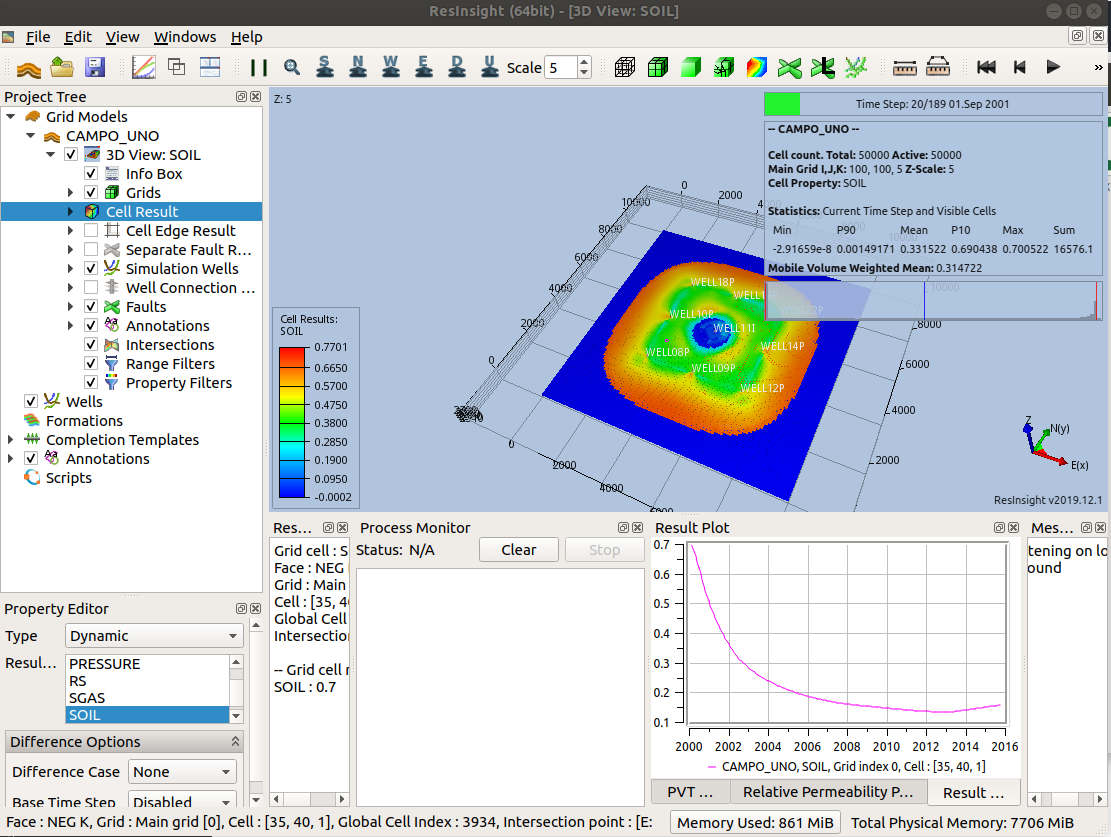
\includegraphics[scale=0.18]{fig/OPM.png}
    \end{center}
\end{columns}
\end{frame}